% Created 2025-02-13 Thu 11:32
% Intended LaTeX compiler: pdflatex
\documentclass[11pt]{article}
\usepackage[utf8]{inputenc}
\usepackage[T1]{fontenc}
\usepackage{graphicx}
\usepackage{longtable}
\usepackage{wrapfig}
\usepackage{rotating}
\usepackage[normalem]{ulem}
\usepackage{amsmath}
\usepackage{amssymb}
\usepackage{capt-of}
\usepackage{hyperref}
\usepackage{listings}
\usepackage{algorithm}
\usepackage{algpseudocode}
\usepackage{amsmath}
\author{Akilan}
\date{\today}
\title{}
\hypersetup{
 pdfauthor={Akilan},
 pdftitle={},
 pdfkeywords={},
 pdfsubject={},
 pdfcreator={Emacs 29.1 (Org mode 9.6.6)}, 
 pdflang={English}}
\begin{document}

\tableofcontents


\section{Fat-pointer Address Translations}
\label{sec:org9194085}

Fat-pointer Address Translations, combined with the capabilities of the CHERI (Capability Hardware Enhanced RISC Instructions) 
architecture, introduce robust memory safety and security features by incorporating additional metadata 
with memory pointers. This enhanced architecture utilizes concepts such as FlexPointer, 
Range Memory Mapping (RMM) to manage memory effectively.

Range addresses play a pivotal role within this implementation, defining memory 
regions bounded by a starting address (Upper) and an ending address (Lower). 
These range addresses are encoded within FAT-pointers, allowing for precise 
control over memory regions.

\begin{figure}[htbp]
\centering
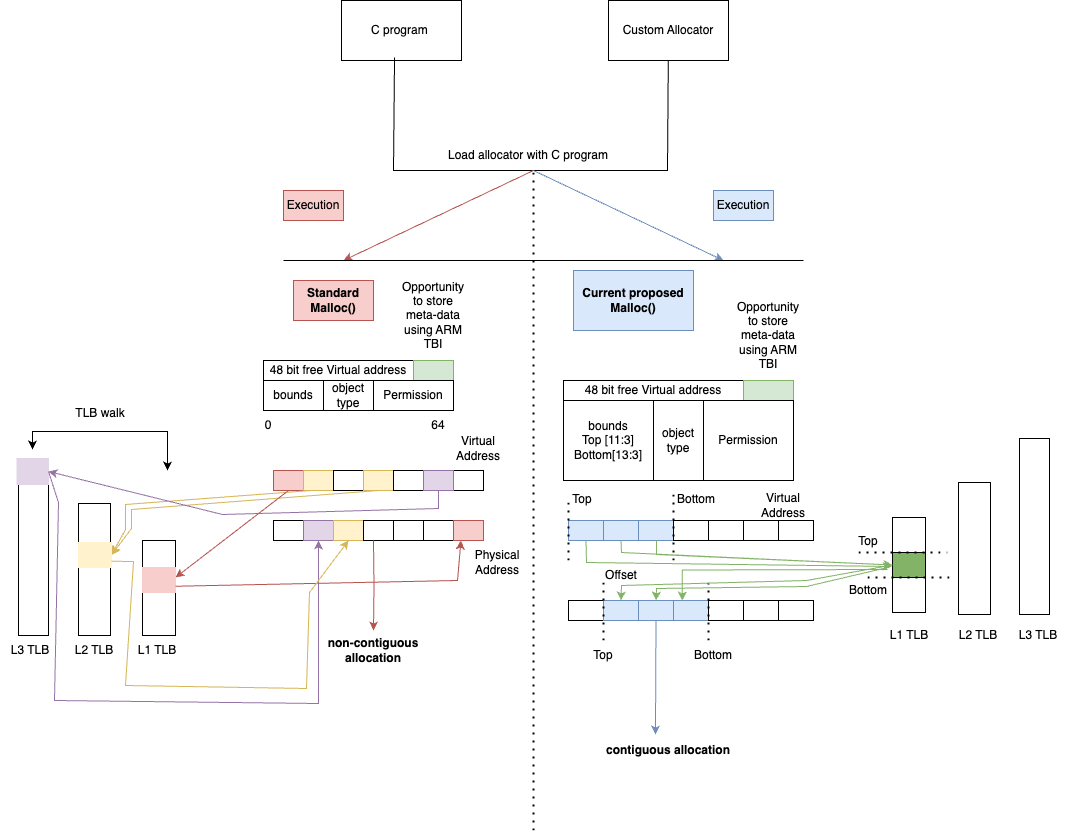
\includegraphics[width=.9\linewidth]{diagram/HighOverviewArchitecture.drawio.png}
\caption{\label{fig:orgcb94e61}High overview architecture}
\end{figure}

Figure \ref{fig:orgcb94e61} illustrates
the methodology employed to leverage the CHERI 
128-bit FAT-pointer scheme for facilitating
block-based memory management on physically
contiguous memory,which is depicted on the
right side of the figure. 
This technique contrasts with the
conventional approach.

We explore how using Huge pages
with CHERI bounds can reduce the
number of TLB entries required. 

The functionality of ranges encompasses
several key aspects:

\subsection{Encoding Ranges as Bounds to the Pointer}
\label{sec:org312bc7d}
\begin{figure}[htbp]
\centering
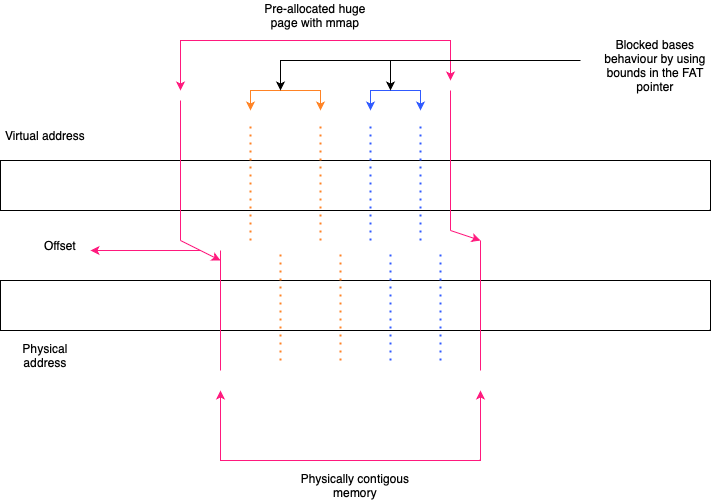
\includegraphics[width=.9\linewidth]{diagram/AllocationOverview24.png}
\caption{\label{fig:org18f47e9}Range of memory}
\end{figure}

Integrating range bounds directly into FAT-pointers enables the architecture 
to enforce memory access restrictions at the pointer level thus allowing 
tracking of memory ranges on a pointer level. In this implementation, memory ranges are established using
bounds encoded within the FAT-pointer, adhering to the CHERI
128-bit bounds compression scheme\cite{woodruff_cheri_2019}.

Figure \ref{fig:org18f47e9} illustrates a straightforward use-case in which the dark pink line represents a single, 
large contiguous memory area, or huge page. Within this huge page, the orange and blue lines indicate 
two separate memory allocations equivalent to invoking malloc twice to allocate memory in distinct regions. 
This scenario simulates a block-based memory allocator operating within the confines of the huge page. 
The allocations leverage the bounds encoded in the FAT-pointer, ensuring tracking and efficient 
management of the allocated memory regions. By using the FAT-pointer bounds, this method maintains the 
integrity and contiguity of the allocated blocks within the huge page.

\subsection{Instrumenting Block-Based Allocators with Physically Contiguous Memory}
\label{sec:orgd7c897c}
\begin{figure}[htbp]
\centering
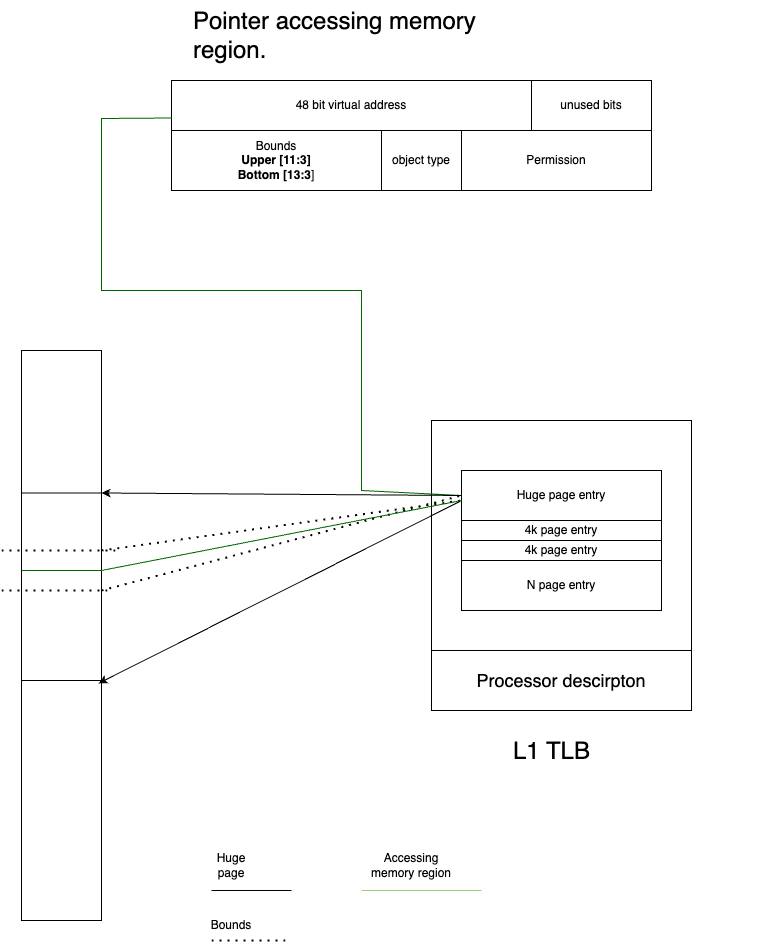
\includegraphics[width=.9\linewidth]{diagram/TLBAccess.drawio.png}
\caption{\label{fig:org710cee0}Fat-pointer Address Translations using huge pages}
\end{figure}

Traditional address translation methods rely on hierarchical
structures to map virtual addresses to physical addresses.
This often requires multiple entries to handle different
memory segments, which increases overhead and adds complexity
to the translation process. In contrast, the current approach
simplifies this by using a single TLB (Translation Lookaside Buffer)
entry to translate multiple addresses within a contiguous memory
range. This reduces the number of TLB entries needed, making the
translation process more efficient and less complex.

By consolidating address translations into a single TLB entry,
this method cuts down on the overhead of managing many entries.
It also takes advantage of the bounds encoded within fat-pointers
to track and access memory more efficiently. This streamlined
approach allows for precise and effective memory management,
especially within large, contiguous memory regions like huge pages.
Overall, it simplifies memory operations while improving performance
and reduces TLB overhead by reducing TLB walks.

Figure \ref{fig:org710cee0} illustrates a use-case of huge pages where the green
line represents a sample access to read within a contigous
space of physical memory. The dotted lines represents the
bounds for that particular pointer access. Using bounds
stored on the pointer a block based pattern can be reprecated
on physically contigous memory. 

\subsection{Sample memory allocator Implementation}
\label{sec:org99d3fdd}
This section presents a straightforward memory allocator designed and implemented based on the 
principles outlined in our approach. The allocator consists of three core functions: InitAlloc, 
malloc, and free. The InitAlloc function initializes the memory pool, setting up the necessary 
data structures and metadata required for efficient memory management. The malloc function is 
responsible for allocating a contiguous block of memory of a specified size, while the free 
function deallocates the memory, returning it to the pool for future use.

A notable feature of this malloc implementation is its compatibility with kernel modules, 
where it can be integrated as an alternative to the mmap system call. This integration 
ensures that memory allocations are physically contiguous, a critical requirement for 
certain low-level operations and hardware interactions. By providing physically contiguous 
memory blocks, this allocator can serve as a foundational layer for standard block-based allocators, 
such as Jemalloc, enabling them to operate efficiently in environments where physical memory 
contiguity is essential.

\begin{algorithm}
\caption{Sample init alloc function to create a initial 1 GB huge page}
\label{alg:initAlloc}
\begin{algorithmic}[1]
\Function{Init\_alloc}{}
    \State $\text{sz} \gets 1\ \text{GB}$ \Comment{Define pre-allocated memory size}
    \State $\text{fd} \gets \text{CREATE\_LARGE\_PAGE\_MEMORY}(\text{sz})$ \Comment{Create shared memory}
    \State $\text{ptr} \gets \text{MAP\_MEMORY}(\text{sz})$ \Comment{Map memory region}
    \State $\text{MallocCounter} \gets \text{sz}$ \Comment{Initialize memory counter}
\EndFunction
\end{algorithmic}
\end{algorithm}

Algorithm \ref{alg:initAlloc} describes the initialization of physically contiguous memory through the use of huge pages,
a mechanism supported by modern architectures to optimize memory management. The algorithm begins by 
allocating a fixed block of 1 GB of physically contiguous memory. This decision is driven by the 
architectural constraints of contemporary systems, particularly ARM-based CPUs, where 1 GB represents 
the largest supported page size. By leveraging huge pages, the algorithm reduces the overhead associated 
with page table management and enhances memory access efficiency, which is critical for performance-sensitive
applications and kernel-level operations.

\begin{algorithm}
\caption{Sample malloc implementation}
\label{alg:malloc}
\begin{algorithmic}[1]
\Function{malloc}{sz}
    \State $sz \gets \text{ALIGN\_UP}(sz, \text{MAX\_ALIGNMENT})$ \Comment{Align size to max alignment}
    \State $\text{MallocCounter} \gets \text{MallocCounter} - sz$ \Comment{Update remaining memory}
    \State $\text{ptrLink} \gets \&\text{ptr}[\text{MallocCounter}]$ \Comment{Calculate pointer address}
    \State $\text{ptrLink} \gets \text{SET\_BOUNDS}(\text{ptrLink}, sz)$ \Comment{Set bounds for memory safety and to track the length of the pointer}
    \State \Return $\text{ptrLink}$ \Comment{Return allocated memory pointer}
\EndFunction
\end{algorithmic}
\end{algorithm}
When the malloc function \ref{alg:malloc} is invoked, the algorithm employs an eager allocation strategy for physical memory. 
This is achieved through the use of the SetBounds mechanism, which constructs a FAT-pointer—a specialized 
pointer that encodes both the start and end addresses of the allocated memory region within the pointer 
itself. The start and end addresses correspond to the size of the memory block requested by malloc. This 
approach introduces a method of memory tracking, where the bounds of the allocated region are 
explicitly encoded in the address, enabling efficient monitoring and management of memory usage.

Furthermore, this design leverages shared huge page TLB (Translation Lookaside Buffer) entries to map 
and track memory addresses. By encoding bounds directly into the address, the algorithm ensures that memory 
accesses remain within the allocated region, thereby enhancing safety and reducing the risk of out-of-bounds 
errors. This use of FAT-pointers and shared TLB entries not only aligns with the principles of 
efficient memory management but also demonstrates a practical usecase of huge pages in CHERI.

\begin{algorithm}
\caption{Sample free implementation}
\label{alg:free}
\begin{algorithmic}[1]
\Function{free}{ptr}
    \State $\text{len} \gets \text{GET\_LENGTH}(\text{ptr})$ \Comment{Get length of memory block from the defined bounds}
    \State $\text{UNMAP}(\text{ptr}, \text{len})$ \Comment{Release memory block}
\EndFunction
\end{algorithmic}
\end{algorithm}

The memory deallocation \ref{alg:free} mechanism in the proposed allocator is facilitated by the FAT-pointer structure 
introduced in the malloc algorithm. When the free function is invoked, it utilizes the metadata 
embedded within the FAT-pointer to determine the range and size of the allocated memory region. 
Specifically, the start and end addresses encoded in the FAT-pointer provide the necessary information 
to identify the exact memory block to be deallocated. This allows the allocator to precisely unmapped 
the corresponding memory region from the address space, ensuring efficient and accurate memory management.

By extracting the bounds and size directly from the FAT-pointer, the free function eliminates the need 
for additional metadata lookups or complex data structures, streamlining the deallocation process. 
This approach not only enhances performance but also reduces the risk of memory leaks or fragmentation.

\bibliographystyle{IEEEtran}
\bibliography{FAT-Pointer.bib}
\end{document}